\section{Evaluation}
\label{sec:eval}

We demonstrate the viability of our proposed scheme using Google Cloud.
We implement an indexing service, a search service and a
client application as standard Java services. We deploy the search service 
on Google App Engine configured as an F4 class instance with a 2.4 GHz CPU and 512
MB of RAM. We utilize Google Blobstore for hosting index files because
it allows us to store and retrieve the complete index files efficiently.
%This is in contrast to Google Datastore whose
%entities can hold only a few bytes of data. As a result, when index entries increase,
%read/write operations on index entries in the Datastore become more costly.
We evaluate the results of our approach on a dataset of 150 documents. 
These documents range in size from 5 MB to 100 MB, containing from 5000 to
129,000 keywords. The keywords are chosen to be at least 8 characters in
length and Porter stemming~\cite{porter} is applied to those keywords.
The client is a Lenovo Thinkpad 430 with a 2.6 GHz Intel Core(TM) i5-332M
CPU and 8 GB of RAM.

%\subsection{Indexing Performance}
%Figure \ref{fig:Index-Generation-Time} shows execution time for the index creation
%and encryption 
%processes over different input dataset sizes 
%using a 64-bit Pascal Paillier key and a 3 KB bloom filter. The graph shows that,
%despite using sliding window bloom filters, 
%both encryption and index creation sizes increase linearly with input dataset size.
%
%\begin{figure}[h!]
%  \centering
%  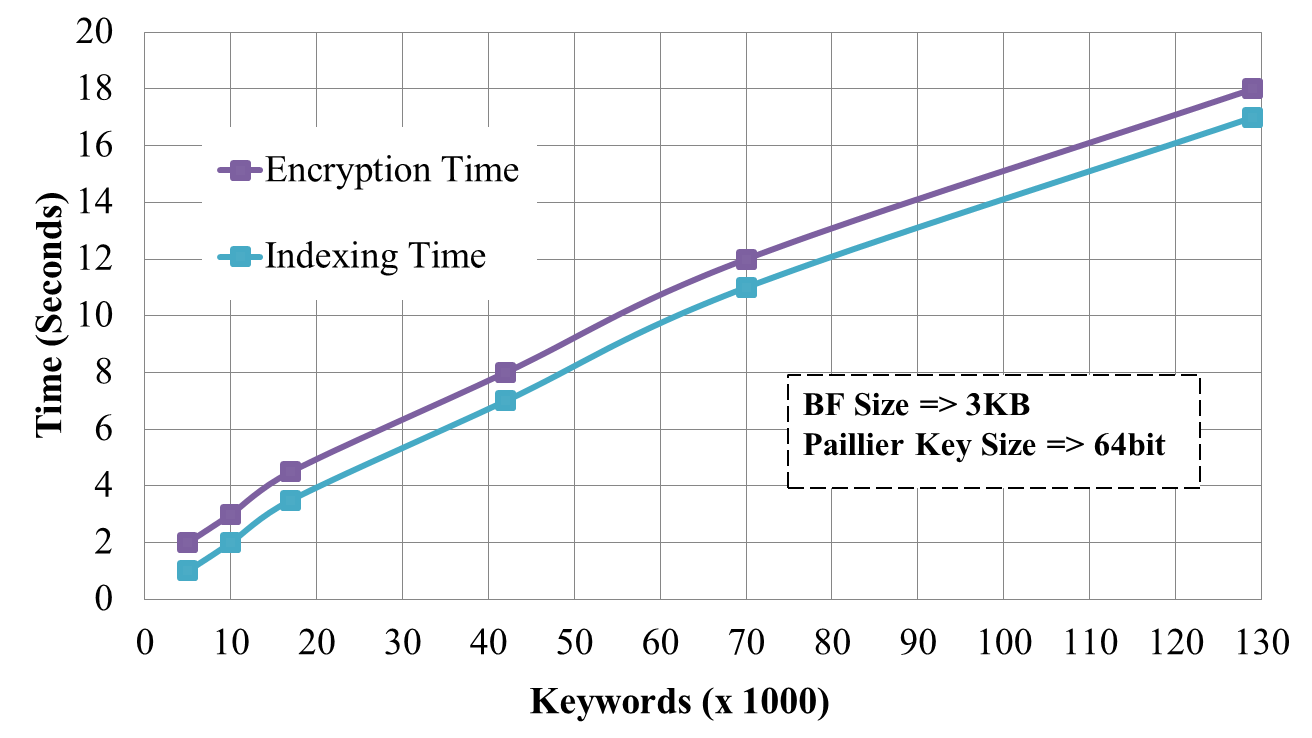
\includegraphics[width=3.5in]{figures/indexing_encryption_time.png}
%  \caption{Index Generation Time}
%  \label{fig:Index-Generation-Time}
%\end{figure}
%
%Paillier key size and bloom filter size both have a substantial impact on index file size. 
%With the increase of bloom filter size, the false positive rate decreases but the size of each
%index entry increases. The indexing time also increases, mainly because it takes longer
%to upload a larger bloom filter to the cloud. 
%A larger Paillier key size can help strengthen system security. However, with
%increasing Paillier key size, index file size also increases proportionally and
%our experiments show that index size increases linearly with Paillier key size.

\subsection{Search Performance}

For private term matching and data returned, our implementation confirms
that our compression algorithm results in 95\% less data returned to the client
compared to traditional approaches, and remains constant even when the size
of the bloom filter increases. This is shown in Figure \ref{fig:compress}.

\begin{figure}[h!]
  \centering
  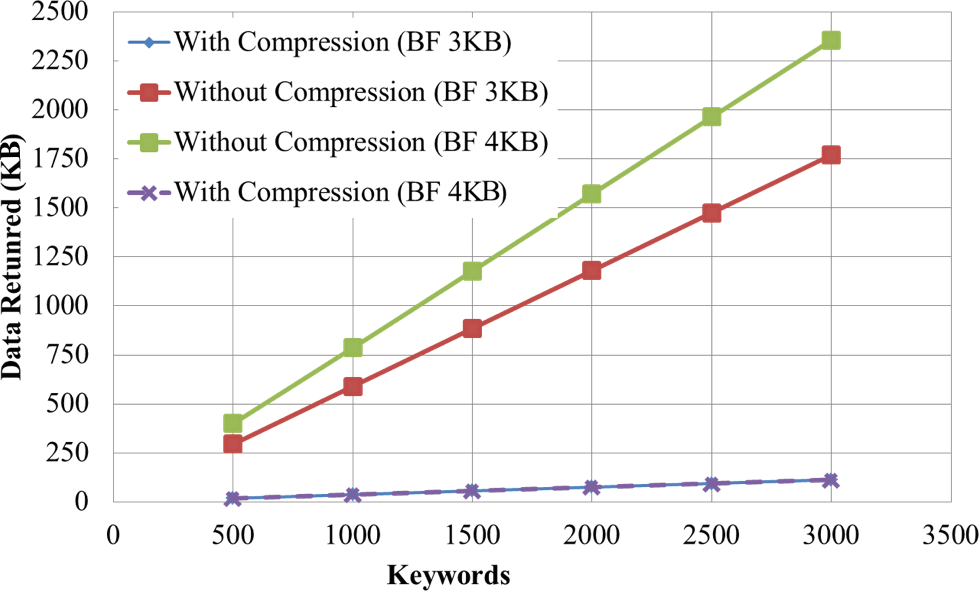
\includegraphics[width=2.7in]{figures/comp_compare.png}
  \vspace{-10px}
  \caption{Data returned by a search query: compressed vs uncompressed results}
  \label{fig:compress}
\end{figure}

%We also measure the time it takes to extract the matching bloom filter values
%from the compressed responses.
%Table \ref{tab:search_response_time} show the results. As expected,
%the extraction time increases linearly with the keyword count
%on the server. 

%\begin{table}[th!]
%\centering
%\caption{Response time increases linearly with keyword count.}
%\label{tab:search_response_time}
%\begin{tabular}{| c | c | }
%\hline
%Keyword Count & Response Extraction Time (ms) \\
%\hline
%500  &  60 \\
%1000 &  125 \\
%1500 &  185 \\
%2000 &  250 \\
%2500 &  310 \\
%3000 &  370 \\
%\hline
%\end{tabular}
%\vspace{-8px}
%
%\end{table}

\subsection{Cost Estimation and Response Times}

Finally, we evaluate the dollar cost that CSP will charge to data owners for search
queries with partial matching. 
Our results, shown in Figure \ref{fig:cost_single_query}, demonstrate that a query
searching for a single keyword in a dataset having 500-3500 index entries will cost only 
\$0.000002 to \$0.00002 per 1000 similar
queries. Due to the sliding window bloom filter approach, 
all of the metrics increase only linearly ($O(n)$) with the number
of keywords on the server. This is substantially better than using a naive algorithm 
for partial matching, which would result in $O(nm)$ time complexity 
for $n$ keywords that are on average $m$ characters long. Crucially,
privacy is preserved throughout the search process because data is never
decrypted at the cloud or by any other untrusted system.


\begin{figure}
  \centering
  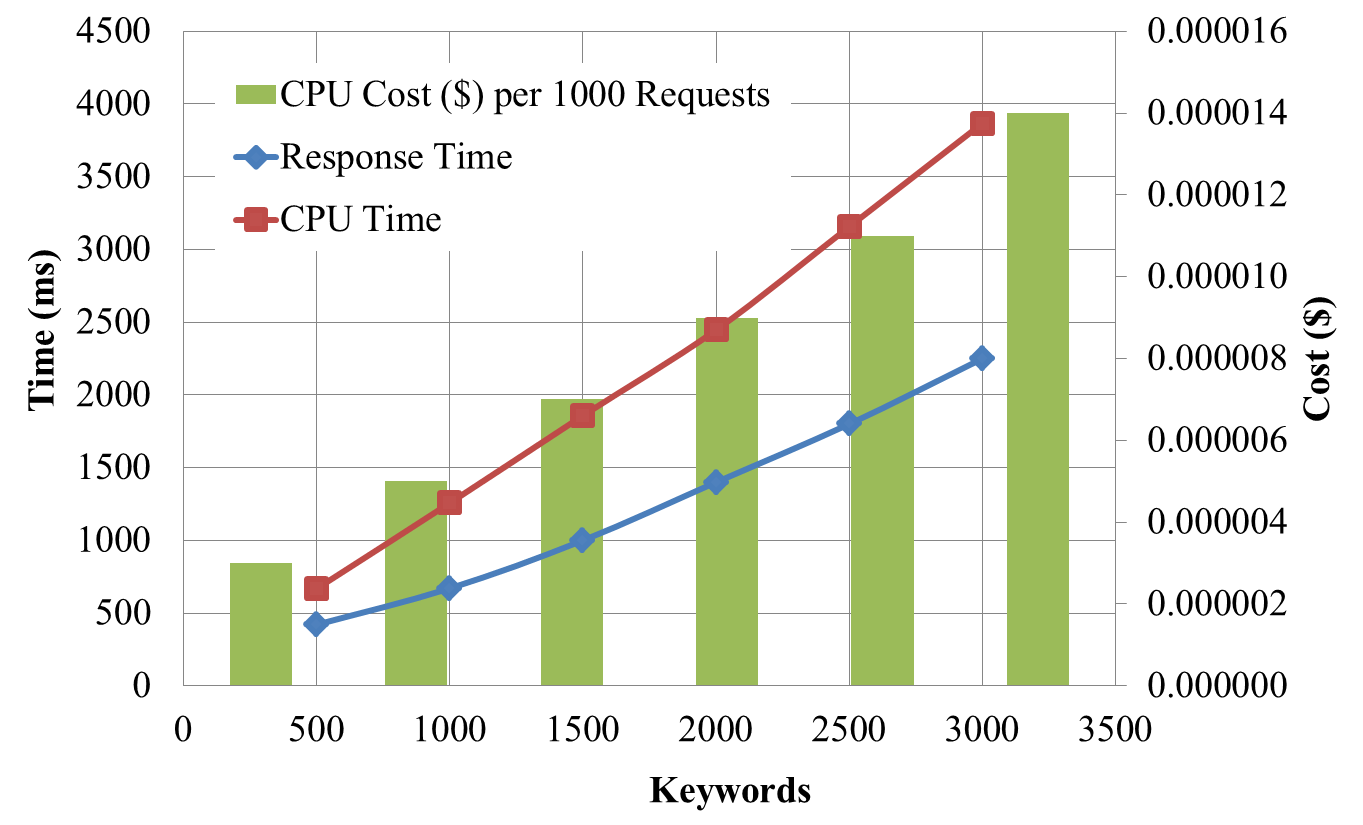
\includegraphics[width=2.7in]{figures/cost_keywords_graph.png}
  \vspace{-10px}
  \caption{Search Cost(\$) with Single Keyword Query}
  \label{fig:cost_single_query}
\end{figure}
